\documentclass[parskip=full]{scrartcl}
\usepackage[utf8]{inputenc} % use utf8 file encoding for TeX sources 

\usepackage[T1]{fontenc} % avoid garbled Unicode text in pdf 
\usepackage[german]{babel} % german hyphenation, quotes, etc 
\usepackage{hyperref} % detailed hyperlink/pdf configuration
\usepackage{graphicx}
\usepackage[toc]{glossaries}
\usepackage{caption}
\hypersetup{ % ‘texdoc hyperref‘ for options 
pdftitle={PSE Pflichtenheft}, %
bookmarks=true,%
}
\usepackage{csquotes} % provides \enquote{} macro for "quotes"
\usepackage{enumitem}




\makeglossaries
\newglossaryentry{Schachregeln}
{
	name=Schachregeln,
	description={Schachregeln die gültige Züge und das Ende des Spiels definieren. \href{https://de.wikipedia.org/wiki/Schach\#Spielregeln}{https://de.wikipedia.org/wiki/Schach\#Spielregeln}}
}

\newglossaryentry{Schach}
{
	name=Schach,
	description={Das Brettspiel Schach}
}

\newglossaryentry{Schachfigur}
{
	name=Schachfigur,
	description={Die Spielsteine auf einem Schachbrett},
	plural=Schachfiguren
}

\newglossaryentry{Schachbrett}
{		
	name=Schachbrett,
	description={Das Spielbrett. Es ist quadratisch, zweifarbig und besteht aus 64 quadratischen Kacheln. Diese besitzen alle dieselbe Größe und sind in waagrechter und senkrechter Richtung abwechselnd eingefärbt},
	plural=Schachbretter
}

\newglossaryentry{Ausgangsposition} 
{
	name=Ausgangsposition,
	description={Vorgeschriebene Startposition aller Spielfiguren zu Beginn jeder Schachpartie}
}

\newglossaryentry{Remis}
{
	name=Remis,
	description={Der unentschiedene Ausgang einer Schachpartie, entweder durch Einigung beider Spieler oder durch Erreichen einer Stellung oder Zugfolge, welche ein Unentschieden erzwingt}
}

\newglossaryentry{Revanche}
{
	name=Revanche,
	description={Spiel, das dem Verlierer einer vorangegangene Partie die Chance gewährt, die Niederlage wieder wett zu machen, hier auch für den Gewinner möglich}
}

\newglossaryentry{Spieler}
{
	name={Spieler},
	description={Ein Nutzer der App},
}

\newglossaryentry{Elo}
{
	name={Elo},
	description={Wertung, die die Spielstärke beschreibt. \href{{https://de.wikipedia.org/wiki/Elo-Zahl}{https://de.wikipedia.org/wiki/Elo-Zahl}}}
}

\newglossaryentry{Schachmatt}
{
	name={Schachmatt},
	description={Der König steht im Schach und es gibt keinen regelkonformen Zug der das Schachgebot aufhebt. \href{https://de.wikipedia.org/wiki/Schachmatt}{https://de.wikipedia.org/wiki/Schachmatt}}
}

\newglossaryentry{Notation}
{
	name=Notation,
	description={Notation zur eindeutigen Dokumentation des Verlaufs einer Schachpartie. 	\href{https://de.wikipedia.org/wiki/Schachnotation}{https://de.wikipedia.org/wiki/Schachnotation}}
}

\newglossaryentry{Bedenkzeit} 
{
	name=Bedenkzeit,
	description={Maximale Zeit die einem Spieler für eine Schachpartie zur Verfügung steht. Es wird immer nur die Bedenkzeit des aktuell zu ziehenden Spielers dekrementiert. Bei Ablaufen seiner Bedenkzeit verliert der Spieler die Partie.}
}

\newglossaryentry{Android}
{
	name={Android},
	description={Ein Betriebssystem für mobile Geräte wie Smartphones, Tablets und auch Fernseher}
}
\newglossaryentry{Smartphone}
{
	name={Smartphone},
	description={Ein Mobiltelefon mit umfangreichen Computer-Funktionalitäten},
	plural = Smartphones
}
\newglossaryentry{Graphical User Interface}
{
	name={Graphical User Interface},
	description={Deutsch: Graphische Benutzeroberfläche}
}
\newglossaryentry{Schach-Engine}
{
	name={Schach-Engine},
	description={Ein Computer Programm zur Berechnung von möglichen Zügen \href{https://de.wikipedia.org/wiki/Schachprogramm}{https://de.wikipedia.org/wiki/Schachprogramm}}
}
\newglossaryentry{Patt}{
	name={Patt},
	description={Patt im Schach tritt auf, falls dem am Zug befindlichen Spieler keine Zugmöglichkeit zur Verfügung steht, sein König sich jedoch nicht im Schach befindet}
}
\newglossaryentry{tote Stellung}{name={tote Stellung},description={Tote Stellung liegt vor, falls eine Stellung entstanden ist, in welcher keiner der Spieler den gegnerischen König mit irgendeiner Folge von regelgemäßen Zügen mattsetzen kann. Zumeist hat hierbei keiner der beiden Spieler genug Figuren übrig, um den anderen Spieler mattsetzen zu können (z. B. König gegen König, König gegen König und Springer, König gegen König und Läufer). Es gibt auch Fälle, in denen etwa aufgrund einer verkeilten Bauernstruktur keiner der Spieler gewinnen kann.}}

\newacronym{GUI}{GUI}{Graphical User Interface}



\begin{document}
	\begin{titlepage}
		\centering
		\vspace*{0.2\textheight}
		{\Large PSE}\\[\baselineskip]
		{\Huge PFLICHTENHEFT}\\[\baselineskip]\par
		{\LARGE Rukiye Devran, Tim Groß, Daniel Helmig, Orkhan Aliev, Florian Weber}\par
	
	\newpage	
	\tableofcontents
	\pagebreak
	
	\end{titlepage}
\section{Zielbestimmung}

\gls{Schach} ist weltweit bekannt und hat über viele Jahre hinweg eine tiefe kulturelle Bedeutung erlangt. Dadurch ist es zu einer Sportart geworden, die viele begeistert.
Deshalb soll im Rahmen der Praxis der Softwareentwicklung eine \gls{Schach}-App entwickelt werden, die es ermöglicht zu jeder Zeit Schach zu spielen.
Spieler sollen Gegner durch eine Spielersuche finden. Außerdem können sie sich in einer Rangliste vergleichen und es wird eine Statistik über jeden Spieler geführt.
Die App soll somit ein \gls{Schach}spiel simulieren, wo man trotz weiter Entfernungen gegeneinander spielen kann, ohne sich gegenüber zu sitzen.
Letztendlich kann man durch häufiges Spielen bessere Spielfähigkeiten erlangen, sich mit anderen Spielern vergleichen und gegen seine Freunde spielen.

\subsection{Musskriterien}
\begin{description}
\item[KM1010] \textbf{\textit{\gls{Schachregeln}}}
\begin{itemize}
	\item Alle \gls{Schachregeln} sollen implementiert werden.
	\item Das Spielende soll definiert sein.	
\end{itemize}
\item[KM1020] \textbf{\textit{Einhaltung der \gls{Schachregeln}}}
\begin{itemize}
	\item Der Nutzer soll nur gültige Züge, die den \gls{Schachregeln} entsprechen, ausführen können.
\end{itemize}
\item[KM1030] \textbf{\textit{Spielersuche}}
\begin{itemize}
	\item Es soll dem Spieler möglich sein mit anderen Spielern zu spielen und zwar:
	\begin{itemize}
		\item Gegen einen zufälligen Gegner
		\item Gegen einen bestimmten Spieler, der mithilfe einer Suchfunktion bestimmt wird.
	\end{itemize}
\end{itemize}
\item[KM1040] \textbf{\textit{\gls{GUI}}}
\begin{itemize}
	\item Die Oberfläche besteht aus:
	\begin{itemize}		
		\item Login Seite: Hier soll sich der Nutzer mit Hilfe eines externen Kontos anmelden können.
		
		\item Hauptmenü: Hier soll der Nutzer dazu in der Lage sein, Spiele zu starten und seine Statistiken aufzurufen.
		
		\item Statistik Seite: Der Nutzer kann seine Spielstatistiken einsehen.
		
		\item Schachbrett: Hier kann der Nutzer in einer Partie seine Züge durchführen.
		
		\item Diverse Meldungen an den Spieler
	\end{itemize}
\end{itemize}
\item[KM1050] \textbf{\textit{\glspl{Schachfigur} bewegen}}
\begin{itemize}
	\item Es muss möglich sein, jede seiner Figuren anzutippen und damit auszuwählen.
	\item Für eine ausgewählte \gls{Schachfigur} müssen mögliche Züge angezeigt werden.
	\item Nur gültige Züge sollen ausgeführt werden können.
\end{itemize}
\end{description}

\subsection{Wunschkritierien}
\begin{description}

	\item[KW1010] \textbf{\textit{Account/Gastzugang}}
	\begin{itemize}
		\item Das Erstellen eines Accounts mit wählbarem und eindeutigen Benutzername soll 		möglich sein.
		\item Außerdem soll es die Möglichkeit geben, ohne Accounterstellung mittels eines 		Gastkontos zu spielen. Der Name wird automatisch vergeben.		
	\end{itemize}
	
	\item[KW1020] \textbf{\textit{Spiel speichern}}
	\begin{itemize}
		\item Beide Spieler sollen ein Spiel nach Beenden der Partie speichern können.
		\item Es soll eine Textdatei mit dem Partieverlauf in algebraischer \gls{Notation} erzeugt und auf dem Mobilgerät abgespeichert werden.
		\item Benutzer können die Textdatei öffnen und die Partie auf einem Brett nachspielen.
	\end{itemize}
	
	\item[KW1030] \textbf{\textit{Einstellbare Bedenkzeit und Spielfarbe}}
	\begin{itemize}
		\item Beide Spieler einer Partie sollen eine maximale Bedenkzeit haben.
		\item Beim Herausfordern eines zuvor gewählten Spielers soll die Bedenkzeit sowie die gewünschte Spielfarbe einstellbar sein.
		\item Zur Wahl der Bedenkzeit soll eine Liste mit möglichen Zeiten erscheinen.
		\item Bei der Farbwahl soll zwischen Weiß, Schwarz und zufällig gewählt werden				können.
	\end{itemize}
	
	\item[KW1040] 
	\begin{itemize} \textbf{\textit{Spielerchat}}
		\item \gls{Spieler} können einen Chat mit dem entsprechenden Gegner führen.
		\item Dazu soll es während einer Partie ein Chatsymbol geben, welches ein Chatfenster öffnet.
		\item Dort können Nachrichten an den Gegner verschickt werden können, sowie Spielmeldungen erscheinen.
	\end{itemize}
	
	\item[KW1050] \textbf{\textit{\gls{Elo}system und Rangliste}}
	\begin{itemize}
	\item Es soll für jeden Spieler eine \gls{Elo}zahl zur Messung der Spielerstärke existieren.
	\item Nach jeder Partie sollen die Werte beider Spieler entsprechend einer Formel aktualisiert werden.
	\item Es soll eine Rangliste existieren, in welcher alle Spieler anhand ihrer \gls{Elo}zahl in absteigender Reihenfolge gelistet werden .
	\end{itemize}
	
	\item[KW1060] \textbf{\textit{Anmeldung mit Facebook oder Google}}
	\begin{itemize}
	\item Benutzer sollen die Möglichkeit haben, sich mit ihrem Google bzw. Facebook-Konto anzumelden.
	\item Der Account ist dann mit dem jeweiligen Konto verknüpft.
	\end{itemize}
	
	\item[KW1070] \textbf{\textit{Zwei Spieler auf einem Gerät}}
	\begin{itemize}
	\item Spieler sollen die Möglichkeit haben, zu zweit auf einem Gerät gegeneinander zu spielen.
	\item Die Symbole der schwarzen Figuren sollen zur besseren Benutzbarkeit auf den Kopf gedreht sein.
	\end{itemize}
	
	\item[KW1080] \textbf{\textit{\gls{Revanche}-Button}}
	\begin{itemize}
	\item Nach Beenden einer Partie sollen beide Spieler die Möglichkeit haben, einen Rückkampf zu fordern.
	\item Akzeptiert der Gegner die Herausforderung, so soll eine neue Partie gestartet werden.
	\item Die Spieler sollen bei der Revanche die jeweils andersfarbigen Spielfiguren zugeteilt bekommen wie bei der vorherigen Partie, die \gls{Bedenkzeit} soll dieselbe sein.
	\end{itemize}
	
\end{description}
\subsection{Abgrenzkriterien}
\begin{description}
\item[KA1010] \textbf{\textit{\gls{Schach-Engine}:}} Es soll keine selbst spielende \gls{Schach-Engine} implementiert werden.
\item[KA1020] \textbf{\textit{Zurücknahme:}} Die Spieler können Züge nicht zurücknehmen.
\item[KA1030] \textbf{\textit{Spielmodi:}} Bei der Spielsuche soll es keine Möglichkeit zur Modifikation des Spielmodus geben.
\item[KA1040] \textbf{\textit{Fremde Partien:}} Spiele von anderen \gls{Spieler}n können nicht live verfolgt werden.
\item[KA1050] \textbf{\textit{Partien einlesen:}} Es soll nicht möglich sein, andere Partien einzulesen.
\item[KA1060] \textbf{\textit{Mehrere Partien:}} Es ist nicht machbar, mehrere Partien gleichzeitig zu spielen.
\item[KA1070] \textbf{\textit{\gls{Bedenkzeit}:}} Der Spieler ist nicht dazu in der Lage, seinem Gegner mehr \gls{Bedenkzeit} zu gewähren.
\end{description}
\newpage
\section{Produkteinsatz}
	\subsection{Anwendungsbereich}
		
			Privatpersonen sollen in der Lage sein mit anderen Personen \gls{Schach} zu spielen. Die Anwendung soll dies schnell, einfach und mobil ermöglichen.	
		
	\subsection{Zielgruppe}
		
			Die Anwendung richtet sich an Personen mit einem Android \gls{Smartphone}, die unterwegs eine Partie \gls{Schach} spielen möchten.
		
	\subsection{Betriebsbedingungen}
		\begin{description}
			\item Die Anwendung soll täglich 24 Stunden verfügbar sein.
			\item Es sollen alle Versionen ab Android 4.4 unterstützt werden.
			\item Der Server soll wartungsfrei laufen.	
		\end{description}
	\newpage
\section{Produktumgebung}
	\subsection{Software}
		\begin{description}
			\item Eine App für Mobilgeräte mit \gls{Android} Betriebssystem ab Version 4.4.
			\item Ein Java Server zur Verwaltung von Partien und Spielsuche.		
		\end{description}
	\subsection{Hardware}
		\begin{description}			
			\item Ein Internetfähiges \gls{Smartphone} mit:
			\begin{itemize}
			\item \gls{Android} Betriebssystem
			\item Touchscreen
			\end{itemize}
		\item Ein virtueller Computer
		\end{description}
\pagebreak		  
\section{Funktionelle Anforderungen}
\subsection{Benutzerfunktionen}
\begin{description}
	\item[F1010] \textbf{\textit{Anmelden: }} Ein \gls{Android} Nutzer der auch einen Google Account besitzt, kann sich auf der Hauptseite der App erfolgreich anmelden. Für die Anmeldung im System sind folgende Angaben erforderlich:
	\begin{itemize}
		\item e-Mail Adresse, die mit Google Konto in Verbindung steht
		\item Google Konto Passwort 
	\end{itemize}  
	\item[F1020] \textbf{\textit{Gastzugang: }} Benutzer die keinen Google Account besitzen, können sich als Gast im System anmelden. Bei der Anmeldung wird ihnen ein eindeutiger Benutzername vom System zugewiesen. 
	\item[F1030] \textbf{\textit{Abmelden: }} Benutzer, die sich bereits mit ihrem Google Account angemeldet haben, können sich wieder vom System abmelden.
	
	\item [F1040] \textbf{\textit{Anzeige des eigenen, persönlichen Profils: }}  Der Benutzer kann sich sein persönliches Profil anzeigen lassen. Dabei sieht er seine Statistiken:

	\begin{itemize}
		\item Wie viele Spiele gespielt wurden
		\item Wie viele Male gewonnen wurde
		\item Wie viele Male verloren wurde
		\item Wie viele Spiele unentschieden gespielt wurden
		\item Elo-Zahl
		
	\end{itemize}
	\item[F1050] \textbf{\textit{Suche nach Benutzern: }} Der Benutzer kann mit der Suchfunktion nach anderen Benutzern des Systems anhand ihres Benutzernamens suchen.
	
	\item[F1060]  \textbf{\textit{Anzeigen der persönlichen Profile anderer Benutzer: }}
	Der Benutzer kann sich die persönlichen Profile von anderen Benutzern anzeigen lassen, wobei er den Benutzernamen und die Statistiken sieht. Die anderen Benutzer können sich genauso sein Profil anzeigen lassen.
	
	\item[F1070] \textbf{\textit{Multiplayer auf einem Gerät: }}  Mit einer Multiplayer Funktion können zwei Spieler auf einem Gerät gegeneinander spielen
	
	\item[F1080] \textbf{\textit{Chatten: }} Spieler können während des Spiels miteinander chatten.	
	
\end{description}

\subsection{Initialisierung}
\begin{description}
	\hypertarget{F2010}{\item[F2010]}\textbf{\textit{Eröffnung 	eines Spieles: }} Der Benutzer kann Spiele suchen, ohne dabei einen anderen Benutzer als Gegner angeben zu müssen. Dann bekommt er vom System einen Gegner zugewiesen, der auch genauso ein Spiel gesucht hat. Die Farbe ist zufällig und es steht eine feste \gls{Bedenkzeit} von 15 Minuten für jeden Spieler.
	\item[F2020] \textbf{\textit{Spieleinstellungen bestimmen: }} Bei der Herausforderung einer bestimmten Person zum Spiel \textbf{\textit{F2050}} kann der Herausforderer folgende
	Spieleinstellungen aufstellen:
	\begin{enumerate}
		\item Zeit
		\item Farbe
	\end{enumerate}
	\item[F2030] \textbf{\textit{Herausfordern: }} Nachdem ein entsprechender Gegner ausgesucht wurde \textbf{\textit{F1050}} kann der Benutzer ihn zum Spiel herausfordern.
	\item [F2040] \textbf{\textit{Akzeptieren einer Herausforderung: }} Der Benutzer kann die Herausforderung zum Spiel \textbf{F2030} annehmen.
	\item [F2050] \textbf{\textit{Ablehnung einer Herausforderung: }} Der Benutzer kann die Herausforderung zum Spiel \textbf{F2030} ablehnen.
	
	
	
	
\end{description}


\subsection{Spielverlauf} 
\begin{description}
	\hypertarget{F3010}{\item[F3010]}\textbf{\textit{Bewegungsmöglichkeiten: }} Der Benutzer kann während des Spiels, falls er dran ist, einen Zug seiner Wahl unter Beibehaltung der Schach Spielregeln ausführen.
	\item[F3020] \textbf{\textit{Unentschieden(Remis) bieten: }} Ein Spieler, der Remis anbieten möchte, tut dies, nachdem er einen Zug auf dem Schachbrett ausgeführt und nachdem seine Uhr angehalten und die des Gegners sich in Gang gesetzt hat.
	\item[F3030] \textbf{\textit{Remis annehmen: }} Der Benutzer kann, wenn ihm Unentschieden angeboten wurde \textbf{F3020}, das Angebot annehmen.
	
	\item[F3040] \textbf{\textit{Remis ablehnen: }} Der Benutzer kann, wenn ihm Unentschieden angeboten wurde \textbf{F3020}, das Angebot ablehnen.
	
	\item[F3050] \textbf{\textit{Unentschieden bleiben: }}
	Ein Spiel bleibt Unentschieden, falls einer von beiden Spielern Remis angeboten und der andere Spieler das Angebot angenommen hat; oder wenn nach Schachregeln eine Remis Situation auftritt:
	\begin{enumerate}
		\item Falls ein \gls{Patt} auftritt
		\item Falls eine \gls{tote Stellung} vorliegt
		\item Wenn eine identische Stellung mit gleichen Zugmöglichkeiten und demselben Spieler am Zug mindestens zum dritten Mal auf dem Schachbrett entstanden ist 
	\end{enumerate}
	
	\item[F3060] \textbf{\textit{Aufgeben: }} Während des Spiels kann jeder Spieler jederzeit aufgeben.
	\item[F3070] \textbf{\textit{Spiel enden: }} Ein Spiel endet, falls einer von beiden Spielern den anderen Schachmatt gesetzt hat, oder eine der Remis Situationen auftritt \textbf{\textit{F3050}}.
	\item[F3080] \textbf{\textit{Rückkampf anbieten: }} Nachdem ein Spiel zu Ende gekommen ist, muss jeder Spieler den anderen Spieler einen Rückkampf anbieten zu können.
\end{description}
\newpage
\section{Nichtfunktionale Anforderungen}
\begin{description}
	
	\item[NF1010] \textbf{\textit{Start der App: }} Das Starten der App soll auf aktuellen Geräten maximal 3 Sekunden dauern. 
	\item[NF1020] \textbf{\textit{Spiel Erstellung: }} Der Erstellungsprozess \hyperlink{F2010}{\textbf{F2010}} einer neuen Partie darf nicht länger als 5 Sekunden dauern.
	\item[NF1030] \textbf{\textit{Ermittlung von Spielzügen: }} Die Ermittlung \hyperlink{F3010}{\textbf{F3010}} an möglichen gültigen Zügen darf nicht länger als 0,1 Sekunden dauern.
	\item[NF1040] \textbf{\textit{Weiterleitung von Nachrichten: }} Die Weiterleitung und Überprüfung einzelner Züge soll auf dem Server nicht länger als 2 Sekunden dauern.
	\item[NF1050] \textbf{\textit{Verlust von Paketen: }} Bei Übertragungen zwischen zwei Geräten sollen keine Pakete unbemerkt verloren gehen.
	\item[NF1060] \textbf{\textit{Manipulation von Nachrichten: }} Nachrichten/Spielzüge sollen unverändert am Empfänger eintreffen. Sollten Änderungen vorgenommen worden sein, soll dies vom Empfänger erkannt werden können.
	\item[NF1070] \textbf{\textit{Wartung: }} Der Server soll wartungsfrei und ohne Neustarts auskommen.

	
\end{description}

\newpage
\section{Produktdaten}

\subsection{System-Daten auf mobilen Geräten}
\begin{description}
	
	\item[PD1010] Die Einstellungen
	\begin{description}
	\item Die Einstellungen beinhalten:
		

	\begin{itemize}
		\item Benutzername
		\item Verbindungsdaten vom Server
		\item Sonstige Einstellungen
	\end{itemize}
\end{description}


\end{description}



\begin{description}
	
	\item[PD1020] Spieldaten von der aktuell laufender Partie
		\begin{description}
	\item Zu den Spieldaten gehört:
		\begin{itemize}
		\item Partiekennung
		\item Aktueller Zustand des Schachbretts	
	\end{itemize}

	
	\end{description}	
\end{description}


\subsection{System-Daten auf zentralem Server}
\begin{description}
	
\item[PD2010] Server-Einstellungen
\item[PD2020] Partie-Informationen
\begin{description} 
	\item Für jede Partie wird folgendes gespeichert:
	\begin{itemize}
		\item Partiekennung
		\item Benutzername beider \gls{Spieler}
		\item Aktueller Zustand des Schachbrettes
		\item Alle bisherigen Züge
	\end{itemize}

\end{description}
\end{description}

\subsection{Benutzer-Daten auf mobilen Geräten}
\begin{description}
\item[PD3010]  Benutzerinformationen
\begin{description} 
	\item Folgende Daten werden über jeden Benutzer gespeichert:
	\begin{itemize}
		\item Benutzername
		\item Eigene Spielstatistiken
	\end{itemize}
	
\end{description}
\end{description}

\subsection{Benutzer-Daten auf zentralem Server}
\begin{description}
	\item[PD4010]  Benutzerinformationen
	\begin{description} 
		\item Folgende Daten werden über jeden Benutzer gespeichert:
		\begin{itemize}
			\item Benutzername
			\item e-Mail-Adresse
			\item Sonstige Informationen von Login Providern
			\item Spielstatistiken
		\end{itemize}
		\item Zusätzlich wird eine globales Rangliste über die besten \gls{Spieler} gespeichert.
	\end{description}
\end{description}
\newpage
\section{\gls{GUI} Entwürfe}
\section{Globale Testfälle}
\begin{description}
	\item[T1010] Ein Android Nutzer öffnet die Applikation und registriert sich im System. \textbf{F1010}
	\item[T1020] Ein bereits registrierter Nutzer meldet sich mit seinen Benutzernamen und seinem Passwort in der Applikation an. \textbf{F1020}
	\item[T1030] Ein bereits registrierter Nutzer meldet sich vom System ab. \textbf{F1030}
	\item[T1040] Ein Gastspieler bekommt vom System einen eindeutigen Benutzernamen. \textbf{F1040}
	\item[T1050] Ein bereits registrierter Benutzer fordert sein Passwort an. \textbf{F1050}
	\item[T1060] Ein bereits registrierter Benutzer ändert sein Passwort. \textbf{F1060}
	\item[T2010] Der Benutzer erzeugt ein neues Spiel. \textbf{F2010}
	\item[T2020] Der Benutzer führt ein schon eröffnetes Spiel fort. \textbf{F2020}
	\item[T2030] Der Benutzer fordert unter Angabe eines gültigen Benutzernamens einen anderen Benutzer heraus. \textbf{F2030}
	\item[T2040] Der Benutzer nimmt die Herausforderung an. \textbf{F2040}
	\item[T2050] Der Benutzer lehnt die Herausforderung ab. \textbf{F2050}
	\item[T2060] Der Benutzer schaut seine Statistiken an. \textbf{F2060}	
	\item[T3010] Der Benutzer macht irgendeinen Zug seiner Wahl, wobei die Schachregeln eingehalten werden müssen \textbf{F3010}
	\item[T3020] Der Benutzer bietet ein Remis an, vorausgesetzt er ist nicht am Zug \textbf{F3020}
	\item[T3030] Der Benutzer akzeptiert ein Remis \textbf{F3030}
	\item[T3040] Der Benutzer lehnt ein Remis ab \textbf{F3040}
	\item[T3050] Der Benutzer tauscht Nachrichten aus \textbf{F3050}
	
\end{description}
\pagebreak
\section{Systemmodelle}
\subsection{Szenarien}
\textbf{Szenario 1: \glqq Spiele gegen zufälligen Spieler\grqq} \\
Max Mustermann möchte eine Runde Schach in seiner Mittagspause spielen. Er holt sein Smartphone aus der Tasche und klickt auf das Appsymbol.
Da er die App noch nie verwendet hat, muss er sich zuerst anmelden. Nachdem er dies getan hat, befindet er sich im Hauptmenü.
Da keiner seiner Kollegen Zeit hat, möchte er gegen einen zufälligen Gegner spielen. Nun klickt er auf \glqq Spiel suchen\grqq und bekommt die Meldung, dass er nun der Spielsuche hinzugefügt wurde.
Nach kurzer Zeit bekommt er einen Gegner zugewiesen und die Partie beginnt. Vor ihm erscheint das \gls{Schachbrett} in seiner \gls{Ausgangsposition}.

Herr Mustermann hat die Farbe Weiß zugewiesen bekommen und sein Gegner Schwarz. Er wählt einen Bauern an und bekommt seine möglichen Züge dieser \gls{Schachfigur} angezeigt.
Max Mustermann macht seinen Zug. Als nächstes zieht sein Gegner. Nun ist er wieder am Zug. Beide ziehen nun immer abwechselnd. Nach 35 Zügen hat Herr Mustermann
seinen Gegner \gls{Schachmatt} gesetzt. Die Partie ist somit beendet und Max Mustermann bekommt die Meldung, dass er gewonnen hat. Ihm steht nun zur Auswahl ob er eine Revanche anbieten möchte, die Partie auf seinem Gerät speichern will, oder einfach nur ins Hauptmenü möchte. Er klickt auf den Button \glqq Zum Hauptmenü\grqq und wird zum Hauptmenü weitergeleitet.

\textbf{Szenario 2: \glqq Spiele gegen einen Freund\grqq} \\
Magnus und Fabiano wollen in ihrer Freizeit gegeneinander Schach spielen, haben aber gerade kein Schachbrett zur Hand. Beide öffnen auf ihren \gls{Android}-Gerät ihre Schach-App, und Magnus klickt auf den Button \glqq Spieler suchen\grqq. Es öffnet sich eine Spielerübersicht mit einer Suchleiste, in welcher er den Spielernamen von Fabiano eingibt. In der Spielerübersicht erscheint Fabianos Profil, welches Magnus anklickt. Daraufhin öffnet sich Fabianos Profilübersicht mit seinen Statistiken. Auf Fabianos Profil betätigt Magnus den Button \glqq Herausfordern\grqq, und es erscheint ein Auswahlfenster. Magnus wählt als \gls{Bedenkzeit} 2 Stunden und die zufällige Farbenverteilung. Fabiano erhält daraufhin eine Mitteilung, dass er von Magnus zu einem Spiel mit \gls{Bedenkzeit} 2 Stunden herausgefordert wurde, und hat die Möglichkeit, dieses anzunehmen oder abzulehnen. Er klickt auf \glqq Annehmen\grqq und beiden Spielern öffnet sich ein \gls{Schachbrett} in \gls{Ausgangsposition}.

Magnus bekommt die schwarzen Figuren zugeteilt, Fabiano die weißen. Nach 115 Zügen ist die Stellung immer noch ausgeglichen und Fabiano klickt auf \glqq Remis anbieten\grqq. Magnus erhält eine Benachrichtigung mit der Möglichkeit, das \gls{Remis} anzunehmen oder abzulehnen. Auch er sieht in der Stellung keine Gewinnmöglichkeit und klickt deshalb auf \glqq Akzeptieren\grqq. Das Spiel wird beendet und die Statistiken beider Spieler werden aktualisiert. Beide Spieler erhalten eine Mitteilung mit der Möglichkeit, eine \gls{Revanche} zu fordern und das Spiel abzuspeichern. Da Magnus das Spiel gerne noch einmal ansehen möchte, klickt er auf \glqq Spiel speichern\grqq und erhält eine Textdatei mit der algebraischen \gls{Notation} der Partie auf sein \gls{Smartphone}.

\textbf{Szenario 3: \glqq Statistiken einsehen\grqq} \\
Magnus behauptet, er wäre ein besserer Spieler als Fabiano. Dieser zweifelt das an, und bittet Magnus, dessen Statistiken mit seinen zu vergleichen. Beide öffnen ihre Schachapp und sind direkt mit ihrem Account angemeldet, da sie dies vorher eingestellt haben. Anschließend klicken sie im Hauptmenü ihrer Schach-App auf \glqq Statistiken\grqq. Sie können nun jeweils ihre Anzahl an gespielten, gewonnenen, remisierten und verlorenen Spielen, sowie ihre \gls{Elo}zahl einsehen. Beide kommen zu dem Schluss, dass Magnus bessere Werte vorzuweisen hat.
\pagebreak
\subsection{Anwendungsfälle}
\begin{enumerate}
 
    \item
	\begin{description}
	\item[Zustand:] Die App ist geschlossen und beendet.
	\item[Aktion:] Die App wird erstmalig geöffnet.
	\item[Reaktion:] Es erscheint ein Fenster zur Eingabe eines Spielernamens.  \\	
	\end{description}
	
	\item
	\begin{description}
	\item[Zustand:] Die App ist geschlossen und beendet.
	\item[Aktion:] Die App wird zum wiederholten Mal geöffnet.
	\item[Reaktion:] Es erscheint das Hauptmenü und der Benutzer ist unter seinem Spielernamen eingeloggt. \\
	\end{description}
	
	\item
	\begin{description}
	\item[Zustand:] Die App befindet sich im Hauptmenü.
	\item[Aktion:] Der Benutzer klickt auf den Button \glqq Statistiken\grqq.
	\item[Reaktion:] Es öffnet sich eine Accountübersicht mit allen gespeicherten Statistiken.  \\
	\end{description}
	
	\item
	\begin{description}
	\item[Zustand:] Die App befindet sich im Hauptmenü.
	\item[Aktion:] Der Benutzer klickt auf den Button \glqq Spiel suchen\grqq.
	\item[Reaktion:] Der Benutzer kommt in eine Warteschlange für suchende Spieler.  \\
	\end{description}
	
	\item
	\begin{description}
	\item[Zustand:] Die App befindet sich im Hauptmenü.
	\item[Aktion:] Der Benutzer klickt auf den Button \glqq Spieler suchen\grqq.
	\item[Reaktion:] Es erscheint eine Spielerübersicht mit Suchmöglichkeit.  \\
	\end{description}
	
	\item
	\begin{description}
	\item[Zustand:] Die App befindet sich im Hauptmenü.
	\item[Aktion:] Der Benutzer klickt auf den Button \glqq Rangliste\grqq.
	\item[Reaktion:] Alle Spieler werden nach \gls{Elo}zahl sortiert aufgelistet.  \\
	\end{description}
	
	\item
	\begin{description}
	\item[Zustand:] Die App befindet sich im Spielersuchmenü.
	\item[Aktion:] Der Benutzer klickt auf einen anderen Spieler.
	\item[Reaktion:] Es erscheint eine Accountübersicht des Spielers mit Möglichkeit zur Herausforderung.  \\
	\end{description}
	
	\item 
	\begin{description}
	\item[Zustand:] Ein Spiel ist am laufen und der Nutzer ist am Zug.
	\item[Aktion:] Der Benutzer klickt auf eine eigene Figur.
	\item[Reaktion:] Es werden alle möglichen Zugfelder markiert.  \\
	\end{description}
	
	\item 
	\begin{description}
	\item[Zustand:] Ein Spiel ist am laufen und der Nutzer ist am Zug.
	\item[Aktion:] Der Benutzer klickt auf eine gegnerische Figur oder ein leeres Feld.
	\item[Reaktion:] Nichts passiert.  \\
	\end{description}
	
	
	\item
	\begin{description}
	\item[Zustand:] Eine \gls{Schachfigur} wurde angeklickt.
	\item[Aktion:] Der Benutzer klickt auf ein markiertes Feld.
	\item[Reaktion:] Die Figur wird gezogen und die Daten an den Server gesendet.  \\
	\end{description}
	
	\item
	\begin{description}
	\item[Zustand:] Eine \gls{Schachfigur} wurde angeklickt.
	\item[Aktion:] Der Benutzer klickt auf ein nicht markiertes Feld.
	\item[Reaktion:] Es passiert nichts, die Figur wird nicht gezogen, die Markierung bleibt.  \\
	\end{description}
	
	\item
	\begin{description}
	\item[Zustand:] Ein Spiel ist am laufen.
	\item[Aktion:] Es wird ein Zug ausgeführt, welcher einen Spieler Matt oder Patt setzt.
	\item[Reaktion:] Es erscheint eine Benachrichtigung, die Elozahlen und Statistiken der Spieler werden aktualisiert.  \\
	\end{description}
	
	\item
	\begin{description}
	\item[Zustand:] Ein Spiel ist am laufen.
	\item[Aktion:] Ein Spieler klickt auf den Button \glqq Aufgeben\grqq.
	\item[Reaktion:] Es erscheint eine Benachrichtigung, die Elozahlen und Statistiken der Spieler werden aktualisiert.  \\
	\end{description}
	
	\item
	\begin{description}
	\item[Zustand:] Ein Spiel ist am laufen.
	\item[Aktion:] Ein Spieler bietet Remis an.
	\item[Reaktion:] Der andere Spieler erhält eine Benachrichtigung mit Auswahlmöglichkeit.  \\
	\end{description}
	
	\item
	\begin{description}
	\item[Zustand:] Remis wurde angeboten.
	\item[Aktion:] Der Spieler klickt auf den Button \glqq Annehmen\grqq.
	\item[Reaktion:] Es erscheint eine Benachrichtigung, die Elozahlen und Statistiken der Spieler werden aktualisiert.  \\
	\end{description}
	
	\item
	\begin{description}
	\item[Zustand:] Remis wurde angeboten.
	\item[Aktion:] Der Spieler klickt auf den Button \glqq Ablehnen\grqq.
	\item[Reaktion:] Die Benachrichtigung schließt sich, der andere Spieler erhält eine Mitteilung.  \\
	\end{description}



\subsection{Anwendungsfalldiagramme} 
		\begin{minipage}{\linewidth}
			\centering
			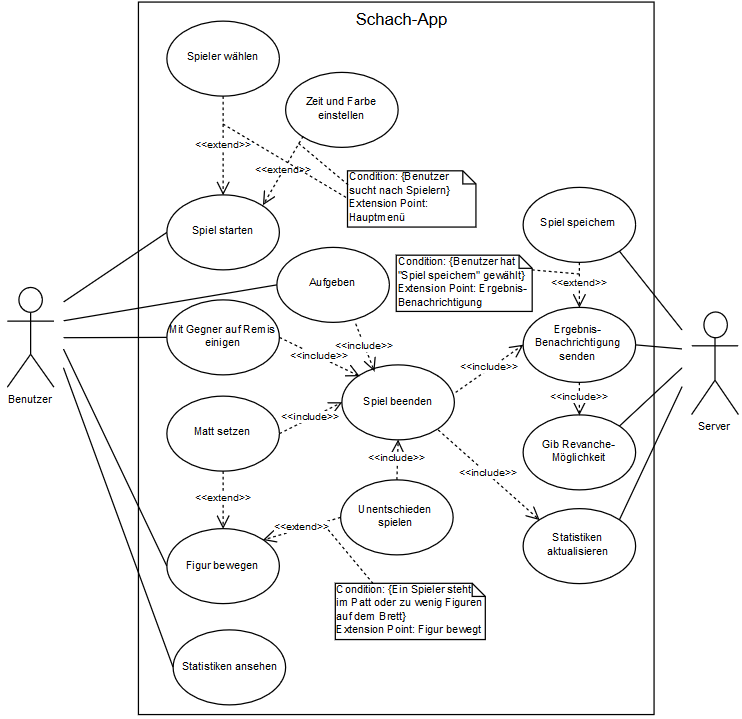
\includegraphics[width=1\linewidth]{Anwendung}
			\label{fig:Schach-App}
				\captionof{figure}{Schach-App}
		\end{minipage}
\end{enumerate}
\pagebreak
\glsaddall 
\printglossaries

\end{document}
